\documentclass{article}
\usepackage[a4paper, portrait, margin=1in]{geometry}
\usepackage{graphicx}
\usepackage{array}
\usepackage{listings}
\usepackage{xcolor}
\usepackage[utf8]{inputenc}
\usepackage{blindtext}
\usepackage[export]{adjustbox}
\usepackage{enumerate}
\usepackage{amsmath}
\usepackage[skip=0.5ex]{subcaption}
\usepackage{caption}
\usepackage{lipsum}
\usepackage{tabularx}
\usepackage{makecell}
\usepackage{subdepth}
\usepackage{cite}

\definecolor{codegreen}{rgb}{0,0.6,0}
\definecolor{codegray}{rgb}{0.5,0.5,0.5}
\definecolor{codepurple}{rgb}{0.58,0,0.82}
\definecolor{backcolour}{rgb}{0.95,0.95,0.92}

\newtheorem{theorem}{Theorem}

\lstdefinestyle{mystyle}{
    backgroundcolor=\color{backcolour},
    commentstyle=\color{codegreen},
    keywordstyle=\color{magenta},
    numberstyle=\tiny\color{codegray},
    stringstyle=\color{codepurple},
    breakatwhitespace=false,
    breaklines=true,
    captionpos=b,
    keepspaces=true,
    numbers=left,
    numbersep=5pt,
    showspaces=false,
    showstringspaces=false,
    showtabs=false,
    tabsize=4
}



\begin{document}

\title{Student Id: 9910821}
\date{}

\maketitle
\section*{Introduction}
This report is a two part study of:
\begin{enumerate}[I)]
  \item Pricing a convertible bond contract in  which, \textbf{at expiry} $T$ the  holder  has  the option to  choose  between  receiving the principle $F$ or alternatively receiving $R$ underlying stocks with price $S$
  \item An extension to the above contract where the holder is able to exercise the decision to convert the bond in stock at \textbf{any time before} the maturity of the contract. Moreover a put option will be embedded in this contract
\end{enumerate}
through the use of advanced numerical methods such as Crank-Nicolson with PSOR and Penalty method.
Particularly, convergence and convergence rates will be studied together with susceptibility to certain algorithmic parameters.

\section{European Type Option Convertible Bond}
The PDE describing such a convertible bond contract is given by
\begin{equation}
  \frac{\partial V}{\partial t} + \frac{1}{2}\sigma^{2}S^{2\beta}\frac{\partial^2 V}{\partial S^2}+\kappa(\theta (t) -S)\frac{\partial V}{\partial S} -rV + Ce^{-\alpha t} =0
  \label{eq:pde_convertible}
\end{equation}

To use advanced numerical methods of (approximately) solving such PDEs we need a numerical scheme. This is a method of rewriting Equation \ref{eq:pde_convertible} as a matrix equation as in Equation \ref{eq:matrix_convertible}.
\begin{equation}
\begin{pmatrix}
b_0 & c_0 & 0 & 0 & . & . & . & . & 0\\[6pt]
a_1 & b_1 & c_1 & 0 & . & . & . & . & .\\[6pt]
0 & a_2 & b_2 & c_2 & 0 & . & . & . & .\\[6pt]
. & . & . & . & . & . & . & . & .\\[6pt]
. & . & . & . & a_j & b_j & c_j & . & .\\[6pt]
. & . & . & . & . & . & . & . & .\\[6pt]
0 & . & . & . & . & . & . & a_{jmax} & b_{jmax}
\end{pmatrix}
\begin{pmatrix}
{V_j^0}\\[6pt]
{V_j^1}\\[6pt]
{V_j^2}\\[6pt]
.\\[6pt]
{V_j^i}\\[6pt]
.\\[6pt]
{V_{jmax}^i}
\end{pmatrix}
=
\begin{pmatrix}
{d_j^0}\\[6pt]
{d_j^1}\\[6pt]
{d_j^2}\\[6pt]
.\\[6pt]
{d_j^i}\\[6pt]
.\\[6pt]
{d_{jmax}^i}
\end{pmatrix}
  \label{eq:matrix_convertible}
\end{equation}
where $j$ represents the steps in $S$ and $i$ the steps in $t$. The Crank-Nicolson method takes approximations of derivatives by Taylor expanding at the half time steps thus yielding
\begin{equation}
  \frac{\partial V}{\partial t} \approx \frac{V_j^{i+1}-{V_j^i}}{\Delta t}
  \label{eq:dvdt}
\end{equation}
\begin{equation}
  \frac{\partial V}{\partial S} \approx \frac{1}{4 \Delta S}(V_{j+1}^{i}-{V_{j-1}^i}+V_{j+1}^{i+1}-V_{j-1}^{i+1})
  \label{eq:dvds}
\end{equation}
\begin{equation}
  \frac{\partial^2 V}{\partial S^2} \approx \frac{1}{2 \Delta S^2}(V_{j+1}^{i}-2{V_{j}^i}+V_{j+1}^{i+1}-2V_{j}^{i+1}+V_{j-1}^{i+1})
  \label{eq:d2vds2}
\end{equation}
\begin{equation}
  V \approx \frac{1}{2}(V_{j}^{i}+{V_{j}^{i+1}}).
  \label{eq:v}
\end{equation}
So substituting Equations \ref{eq:dvdt} - \ref{eq:v} into Equation \ref{eq:pde_convertible} gives the numerical scheme for the non-boundary regime $1 \leq j < jmax$ .
\begin{equation}
  a_j = \frac{\sigma^{2}S^{2\beta}}{4\Delta S^2} - \frac{\kappa(\theta-S)}{4 \Delta S}
  \label{eq:aj}
\end{equation}
\begin{equation}
  b_j = \frac{1}{\Delta t} - \frac{\sigma^2S^{2\beta}}{2 \Delta S^2} - \frac{r}{2}
  \label{eq:bj}
\end{equation}
\begin{equation}
  c_j =\frac{\sigma^{2}S^{2\beta}}{4\Delta S^2} + \frac{\kappa(\theta-S)}{4 \Delta S}
  \label{eq:cj}
\end{equation}
\begin{equation}
  d_j = -\frac{V_{j}^{i+1}}{\Delta t} - \frac{\sigma^2S^{2\beta}}{4 \Delta S^2}(V_{j+1}^{i+1}-2V_{j}^{i+1}+V_{j-1}^{i+1}) - \frac{\kappa(\theta-S)}{4\Delta S}(V_{j+1}^{i+1}-V_{j-1}^{i+1})+\frac{r}{2}V_j^{i+1}-Ce^{-\alpha t}
  \label{eq:dj}
\end{equation}
The boundary conditions are problem dependent so for this particular we have two boundaries at $S=0$ and \({\lim}_{S \to +\infty}\).
Consider the first boundary, when $S=0$ i.e $j=0$. Using Equations \ref{eq:dvdt} and \ref{eq:v} and a modified Equation \ref{eq:dvds} which becomes
\begin{equation}
  \frac{\partial V}{\partial S} \approx \frac{1}{\Delta S}(V_{j+1}^{i}-{V_{j}^i}).
  \label{eq:modified_dvds}
\end{equation}
The numerical scheme after substituing the approximated derivates is now given by
\begin{equation}
  a_0 = 0
  \label{eq:a0}
\end{equation}
\begin{equation}
  b_0 = -\frac{1}{\Delta t} - \frac{\kappa\theta}{\Delta S} - \frac{r}{2}
  \label{eq:b0}
\end{equation}
\begin{equation}
  c_0 =\frac{\kappa\theta}{\Delta S}
  \label{eq:c0}
\end{equation}
\begin{equation}
  d_0 = (-\frac{1}{\Delta t}+\frac{r}{2})V_{j}^{i+1}-Ce^{-\alpha t}
  \label{eq:d0}
\end{equation}
For the \({\lim}_{S \to +\infty}\) we have the condition that
\begin{equation}
  \frac{\partial V}{\partial t} +\kappa(X -S)\frac{\partial V}{\partial S} -rV + Ce^{-\alpha t} =0
  \label{eq:large_s_boundary}
\end{equation}
with the ansatz
\begin{equation}
  V(S,t)=SA(t)+B(t).
  \label{eq:ansatz}
\end{equation}
It can be shown by partial differentiation and integrating using an integrating factor method that
\begin{equation}
  A(t)=Re^{(\kappa+r)(t-T)}
  \label{eq:A}
\end{equation}
and\begin{equation}
  B(t)=-XRe^{(\kappa+r)(t-T)}+\frac{C}{\alpha+r}e^{-\alpha t}-\frac{C}{\alpha+r}e^{-(\alpha+r)T+rt}+XRe^{r(t-T)}.
  \label{eq:B}
\end{equation}
Finally we have the last part of the numerical scheme as
\begin{equation}
  a_0 = 0
  \label{eq:amax}
\end{equation}
\begin{equation}
  b_0 = 1
  \label{eq:bmax}
\end{equation}
\begin{equation}
  c_0 =0
  \label{eq:cmax}
\end{equation}
\begin{equation}
  d_0 = SA(t)+B(t).
  \label{eq:dmax}
\end{equation}
Using this complete numerical scheme, the method is to solve backwards in time from $i=imax$ to $i=0$ where at each time step the Equation \ref{eq:matrix_convertible} is solved using
a method such as Successive Over Relaxation (SOR) for $j=0\to jmax$.
\par\noindent\rule{\textwidth}{0.4pt}
\subsection{Investigating $\beta$ and $\sigma$}
For the rest of this section assume these values were used unless otherwise specified:
$T=2$, $F=95$, $R=2$, $r=0.0229$, $\kappa=0.125$, $\mu=0.0113$, $X=47.66$, $C=1.09$, $\alpha=0.02$, $\beta=0.486$ and $\sigma=3.03$.
For the SOR method a value of $\omega=1.4$ was used with a maximum cap of iterations of 100,000.
The value of the option $V(S,t)$ was investigated as a function of the initial underlying asset
price $S_0$ for two cases:
\begin{enumerate}[1)]
  \item ($\beta=1$, $\sigma=0.416$) with all other parameters as previously defined
  \item ($\beta=0.486$, $\sigma=3.03$) with all other parameters as previously defined
\end{enumerate}
\par The Crank-Nicolson method with the numerical scheme as calculated previously, combined with a SOR iterative method of solving the matrix equation, was implemented in code.
This produced the plots seen in Figure \ref{fig:varying_s}.
\begin{figure}[!t]
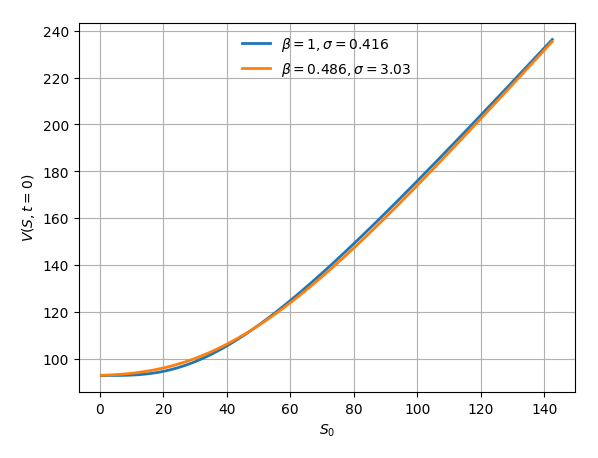
\includegraphics[width=0.5\textwidth,center]{../images/european_varying_s.png}
\caption{Value of the convertible bond $V(S,t=0)$ against inital underlying asset price at time $S_0$ for two combinations of $\beta$ and $\sigma$.}
\label{fig:varying_s}
\end{figure}
The two configurations were therefore found to have the same effect and produce plots for the price of the bond which were very close.
This prompted further analysis on the linked relationship between $\beta$, $\sigma$ and $V(S,t)$.
A 3D graph of the value of the portfolio for a particular $S_0$, here chosen to be equal to $X$, and the two other parameters was plotted.
\begin{figure}[!bh]
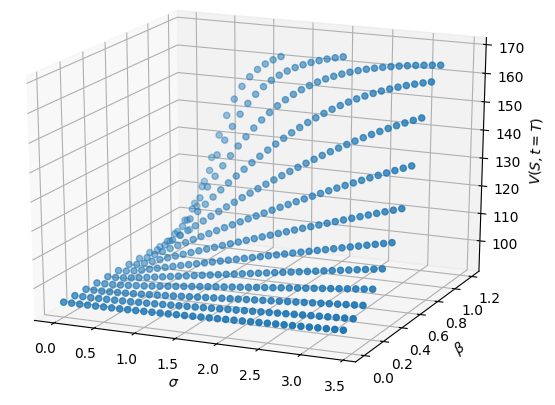
\includegraphics[width=0.55\textwidth,center]{../images/3d_european_varying_s_varying_sigma_varying_beta.png}
\caption{Value of the convertible bond $V(S=X,t=T)$ against parameters $\beta$ and $\sigma$.}
\label{fig:3d_relationship}
\end{figure}
\\
\par Figure \ref{fig:3d_relationship} illustrates such a relationship which is interesting both in shape and in what it can be modelled by.
Going back a few steps, the risk-neutral process followed by the underlying stock price is given by
 \begin{equation}
  dS = \kappa ( \theta (t)-S)dt+\sigma S^{\beta}dW
  \label{eq:process}
\end{equation}
which is an Ornstein-Uhlenbeck (OU) process \cite{thierfelder2015trending} with a drift term of function $\theta(t)$ , together with a Constant Elasticity of Variance \cite{cev} model where the local variance is a powerlaw of elasticity.
Using this model, $\sigma$ is defined to be the actual Black-Scholes volatility or standard deviation of the underlying asset, while $\beta$ is the elasticity parameter of the local volatility.
Moreover, using this model the values of $\beta$ which should be used are for $\leq1$.
Above this, there are implications on the inaccessibility of the origin which for a stock price means it cannot go bankrupt which is not true for stocks or convertible bonds but true for certain commodities such as gold.
Thus, we shall stick for values of $\beta\leq1$ in this report.
In this regime, the model captures the so-called 'leverage effect' where the stock price and volatility are inversely proportional \cite{chan}.
The parameter $\beta$ in Equation \ref{eq:process} controls the steepness of the implied volatility skew which is something seen in Figure \ref{fig:3d_relationship}.
The parameter $\sigma$ is now part of a scale parameter which fixes the 'at-the-money' ($S$ close to $X$ regime) volatility level.
This happens since the variance of the underlying is given by Var(S) $\propto S^{2\beta}\sigma^{2} $.
So, there are $\sigma-\beta$ planes on Figure \ref{fig:3d_relationship} which have close values of the convertible bond for multiple combinations of ($\sigma$ , $\beta$).
\subsection{Varying step sizes}
\begin{figure}[!h]
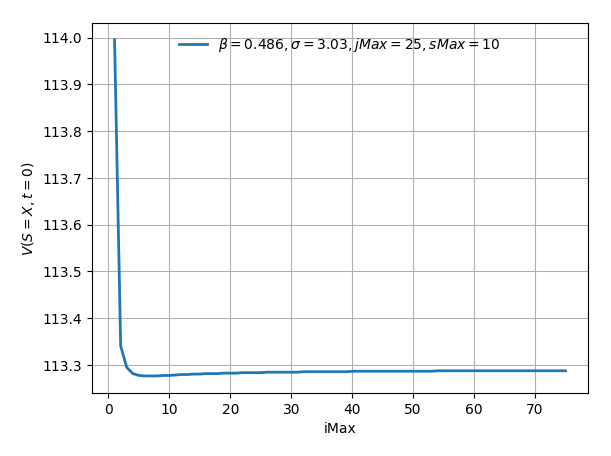
\includegraphics[width=0.5\textwidth,center]{../images/european_varying_imax.png}
\caption{Trend of the convertible bond $V(S=X,t=T)$ as parameter $i_{max}$ is varied.}
\label{fig:varying_imax}
\end{figure}
Finally, for this section the parameters $i_{max}$, $j_{max}$ and $S_{max}$ were investigated to study how a variation in their value affected the result.
The region selected was the at-the-money $S=X$ region of stock price to have comparable results across all three parameters.
Starting with the variation in the time steps, Figure \ref{fig:varying_imax} illustrates such relationship.
Here, it is clear that increasing $i_{max}$ rapidly converges towards a single value of $V(X,T)$ and after $i_{max}=25$ there is really no point in increasing this parameter too much.
\begin{figure}[!th]
\centering
\begin{subfigure}{0.45\textwidth}
    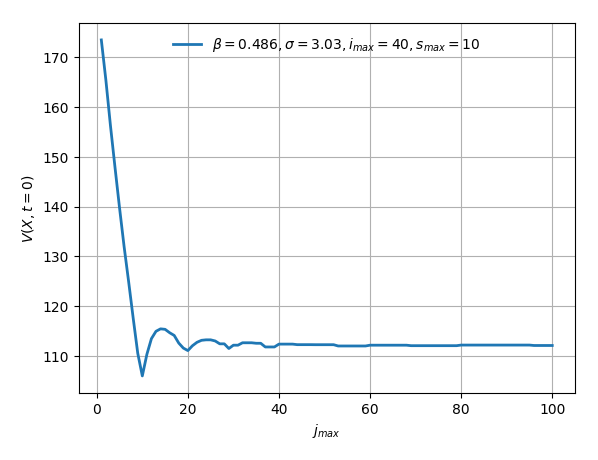
\includegraphics[width=\linewidth]{../images/smax_jmax/10_european_varying_jmax.png}
    \subcaption{Stability and convergence can be obverved after $j_{max}=40$\\}
    \label{fig:varying_jmax_10}
\end{subfigure}
\hfil
\begin{subfigure}{0.45\textwidth}
    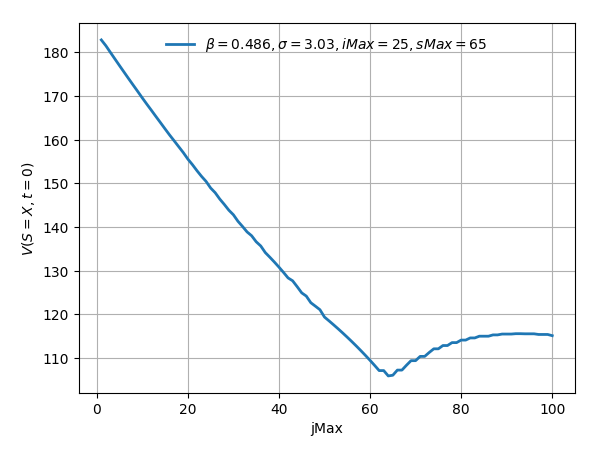
\includegraphics[width=\linewidth]{../images/smax_jmax/65_european_varying_jmax.png}
    \subcaption{The plot from \ref{fig:varying_jmax_10} is stretched and since $S_{max}$ is x6.5 as much, the first minimum is also stretched by that much.}
    \label{fig:varying_jmax_65}
\end{subfigure}
\caption{Plots of the price of the convertible bond $V(X,T)$ against changing $j_{max}$ for different values of $S_{max}$.}
\label{fig:varying_jmax}
\end{figure}
\\
\par When it came to varying $j_{max}$ which is the number of steps in $S$ per timestep, it was noticed
that since the stepsize in $S$ is calculated by dividing $S_{max}$ by the number of steps then these had to go
hand in hand when varying one of them.
Figure \ref{fig:varying_jmax} illustrates this very clearly.
Keeping the range of $j_{max}$ the same and increasing $S_{max}$ shows the same plot but being stretched out in the x-axis.
\\
\par This happens since increasing the maximum cutoff $S$ from which to start at each timestep but keeping the number of steps constant would mean larger jumps
thus a less accurate result everytime.
Instead, ensuring that the overally stepsize in $S$ is constant or small enough is paramount in keeping the result accurate.
Recall that the error in the Crank-Nicolson method is $\mathcal{O}({\Delta S}^2,{\Delta t}^2)$.
Moreover, from these plots we can infer that increasing $S_max$ is pointless (performance-wise) beyond a certain point since we will get the same result by taking more time.
\\
\par
The last issue left to investigate was the time requirements and processing complexity of varying these parameters.
As can be infered from Figure \ref{fig:varying_smax} $i_{max}$ follows a linear time increase while $j_{max}$ is much higher order.
This is because of the fact that a single loop from time $t=T$ to $t=0$ is done but a further loop of $j_{max}$ length is done per time step.
Since the error of Crank-Nicolson is given by $\mathcal{O}({\Delta S}^2,{\Delta t}^2)$ both quantities are important and are dependent directly on $i_{max}$ and $j_{max}$.
\begin{figure}[!h]
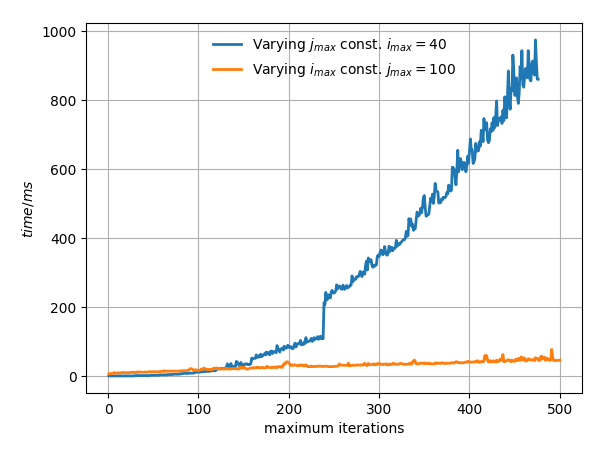
\includegraphics[width=0.5\textwidth,center]{../images/european_time.png}
\caption{Variation of the time required to calculate the convertible bond price as $j_{max}$ and $i_{max}$ are varied.}
\label{fig:varying_smax}
\end{figure}
\\
\par Table \ref{table:euro_convergence} shows the converging trend and rates of convergence for the algorithm used.
The convergence rate is linear with timescale (unlike quadratic as expected from Crank-Nicolson)
and reflects upon the fact that this contract is more complex than, for example, a simple American option.
Errors such as interpolation (here linear was used since Lagrange with $n=4$ was found to be problematic at higher values of $N$) could be the source of such a worse convergence rate than expected.
\begin{table}[!h]
\centering
\begin{tabular}{c|c c c c|}
$N$ & $V(X,0)$ & Iters & Diff.Ratio & Time(ms)\\
\hline
100 & 112.1147738  & 3791 &   &  17 \\
200 & 112.1652622  & 4320 &   &  63 \\
400 & 112.1657249  & 5410 & 109 &  239 \\
800 & 112.1659555  & 7440 & 2.01 &  1023 \\
1600 & 112.1660718  & 11430 & 1.98 &  3896 \\
3200 & 112.1661302  & 26950 & 1.99 &  15129 \\
\hline
\end{tabular}
\caption{Table showing convergence results and rates of PSOR method with
a Crank-Nicolson numerical scheme. Here, $j_{max}=i_{max}=N$ and $S_{max}=N X/30$}
\label{table:euro_convergence}
\end{table}
\\
\par Thus, the final value for $\sigma=3.03$ and $\beta=0.486$ was calculated to be $V(S=X,t=0)=112.166$ with $S_{max}=58X$, $j_{max}=800$, $i_{max}=800$.
\section{American Type Option Convertible Bond with Embedded Option}
\begin{figure}[!h]
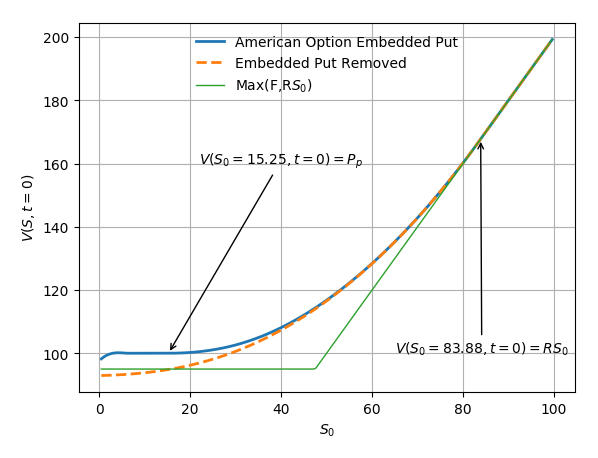
\includegraphics[width=0.65\textwidth,center]{../images/american_varying_s.png}
\caption{Value of the american type option convertible bond $V(S,t=0)$ against inital underlying asset price $S_0$ with and without the embedded put option.}
\label{fig:american_varying_s}
\end{figure}
For this section the numerical method used was Crank-Nicolson Method with Penalty method and Thomas method for the matrix equation solver.
The extension to the european option type convertible bond detailed in Section 1 is to change it to an American type option.
By this we mean that the holder has the option to convert the bond in stock at any time before the maturity of the contract.
To ensure this, the inequality
\begin{equation}
  V \geq RS
  \label{eq:inequality}
\end{equation}
must hold for all $t<T$.
This means the $V_{american}>V_{european}$.
A last addition is to embed a put option in this contract which means the holder has the option to sell the bond back to the issuer over some time period such that
\begin{equation}
  V(S,t) \geq P_p \hspace{15pt} \text{for} \hspace{15pt} t \leq t_0
  \label{eq:inequality_2}
\end{equation}
must hold.
\\
\par Figure \ref{fig:american_varying_s} shows the results of adding these conditions in the code.
The limit for large $S$ is observed as expected to tend to $RS$ and compared to Figure \ref{fig:varying_s} the value of the option is higher.
This is due to the fact that the effective increase in power given to the holder increases the price.
Furthermore, adding the put option increases further the price since again this gives more power to the holder.
This put option might be a sort of safety net in case the value of the stock decreases too much and as with most financial contracts, a decrease in risk must increase the price.
The bond floor is thus observed to be raised when compared to the no-option case.
\\
\par Finally, the arrows are pointing to two decision points at which the price of the contract becomes more than $P_p$ thereafter and becomes more than $RS_0$ thereafter, respectively.
These are important points since the holder would only ever buy the contract for values of $S_0$ between those two points otherwise they would just buy the contract to sell it again or would buy the underlying equity.
\\
\par The sensitivity to the mean reversion rate \cite{CHOUDHRY2001873} $\kappa$ was studied.
Refering back to Equation \ref{eq:process}, this is the rate at which the stock will revert back to the long term mean price described by $\theta(t)$.
As can be seen from Figure \ref{fig:american_varying_s_varying_k} an increase in $\kappa$ decreases the value of the bond in the at-the-money region of the underlying stock.
This is expected since less fluctuations in the stock price movements make it less attractive to buy this contract due to the probabilities of the stock price changing drastically in the future being lower thus the convertibility of the bond being unused.
\begin{figure}[!th]
\begin{minipage}{.5\textwidth}
  \centering
  \begin{subfigure}{\textwidth}
      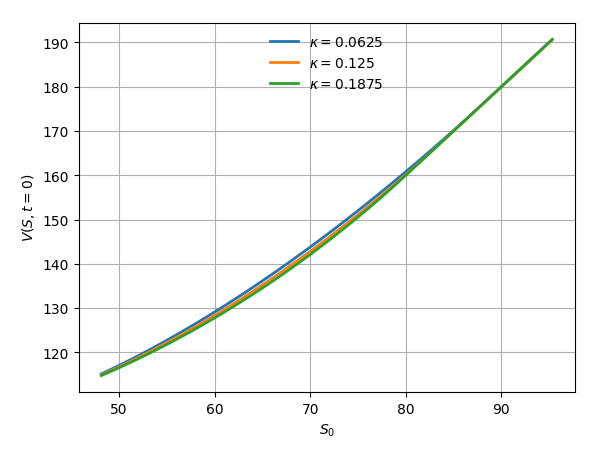
\includegraphics[width=\textwidth,center]{../images/complete_american_varying_s_varying_k.png}
  \end{subfigure}
\end{minipage}
\begin{minipage}{.5\textwidth}
  \centering
  \begin{subfigure}{\textwidth}
      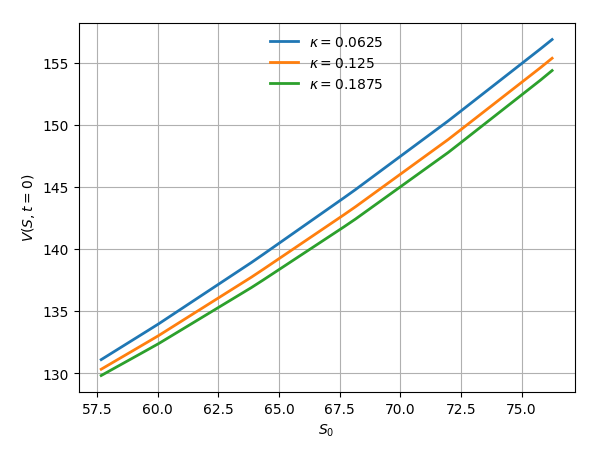
\includegraphics[width=\textwidth,center]{../images/american_varying_s_varying_k.png}
  \end{subfigure}
\end{minipage}
\caption{Value of the american type option convertible bond $V(S,t=0)$ with embedded put option for different values of parameter $\kappa$. Right side plot is a zoomed version of the left side plot.}
\label{fig:american_varying_s_varying_k}
\end{figure}
\\
\par Lastly, it was requested to obtain the most accurate value possible in one second of processing.
Referring to accuracy first, the important thing to eliminate is any source of error.
There are errors on the boundary (finite-element) and errors in discontinuities of the domain.
Interpolation errors were minimised by using Lagrange interpolation of order 4.
Since there is a discontinuity at time $t_0$ one must change the timestep used before and now split the domain effectively in two.
The timestep was chosen such that
\begin{equation}
  \Delta t = \frac{T-t_0}{i_{max}f} \hspace{15pt} \text{for} \hspace{15pt} t_0 < t \leq T
  \label{eq:timestep1}
\end{equation}
\begin{equation}
  \Delta t = \frac{t_0}{i_{max}(1-f)} \hspace{15pt} \text{for} \hspace{15pt} 0 < t \leq t_0
  \label{eq:timestep2}
\end{equation}
where $f=\frac{T-t_0}{T}$.
A better timestepping system would have been Rannacher smoothing \cite{forsyth2002quadratic} however this was beyond the scope of the analysis and as such
literature was used to check that the expected convergence ratios were in the right ranges.
The results, comparing the method PSOR to the penalty method are detailed in Table \ref{table:american_comparison}.
\begin{table}[!h]
\centering
\begin{tabular}{c|c c c c|c c c c|}
 &\multicolumn{4}{c}{Penalty}&\multicolumn{4}{c}{PSOR} \\
\cline{2-5}
\cline{6-9}
\makecell{$N$} & $V(X,0)$ & Iters & Diff.Ratio & Time(ms) & $V(X,0)$ & Iters & Diff.Ratio & Time(ms)\\
\hline
100 & 114.5317065  & 126 &   &  11 & 114.5283612 & 4606 &  & 22 \\
200 & 114.5067677  & 225 &   &  34 & 114.5034113 & 5280 &  & 56 \\
400 & 114.4891972  & 427 & 1.42 &  130 & 114.4858357 & 6389 & 1.42& 163 \\
800 & 114.4804949  & 827 & 2.02 &  554 & 114.4771308 & 8780 & 2.02& 516 \\
1600 & 114.4776084  & 1627 & 3.01 &  1594 & 114.474243 & 12808 & 3.01& 1967 \\
3200 & 114.476139  & 3227 & 1.96 &  6210 & 114.4727731 & 19206 & 1.96& 6599 \\
6400 & 114.4753978  & 8838.6 & 1.98 &  24269 & 114.4720314 & 28648 & 1.98& 24556 \\
\hline
\end{tabular}
\caption{Table comparing convergence results and efficiencies of PSOR and Penalty methods with
a Crank-Nicolson numerical scheme. Here, $j_{max}=i_{max}=N$ and $S_{max}=N X/30$.
Important to note here is the amount of time and iterations saved via the Penalty method.}
\label{table:american_comparison}
\end{table}
\\
\par The results show the convergence rate is nowhere near square with timestep as it should be
for a crank nicolson scheme but rather linear.
This is may be due to the increased complexity the convertibility in the whole life of the
bond brings with it.
Because of the smoothing method taken combined with other errors such as interpolation errors
the rate is less than optimal however it is within expected ranges \cite{li2005pricing}.
Finally, using the information from Table \ref{table:american_comparison} the most accurate value in the given time was found to be:
$V(X,t_0=0)=114.479937$ in $965$ms with $j_{max}=i_{max}=1300$ and $s_{max}=30X$.
\bibliography{references}
\bibliographystyle{ieeetr}
\clearpage
\section*{Appendix 1: European Type Option Code}
\lstset{style=mystyle}
\subsection*{Portfolio Pricing Program Listing}
\lstinputlisting[language=C++]{../european_assignment_4.cpp}
\subsection*{Graphing Program Listing}
\lstinputlisting[language=Python]{../european_assignment_4.py}
\clearpage
\section*{Appendix 2: American Type Option Code}
\lstset{style=mystyle}
\subsection*{Portfolio Pricing Program Listing}
\lstinputlisting[language=C++]{../american_assignment_4.cpp}
\subsection*{Graphing Program Listing}
\lstinputlisting[language=Python]{../american_assignment_4.py}
\end{document}